\documentclass[a4paper]{article}
\usepackage[a4paper, margin=1in]{geometry}
% Some basic packages
\usepackage[utf8]{inputenc}
\usepackage[T1]{fontenc}
\usepackage{textcomp}
\usepackage[dutch]{babel}
\usepackage{url}
\usepackage{graphicx}
\usepackage{float}
\usepackage{booktabs}
\usepackage{enumitem}

\pdfminorversion=7

% Don't indent paragraphs, leave some space between them
\usepackage{parskip}

% Hide page number when page is empty
\usepackage{emptypage}
\usepackage{subcaption}
\usepackage{multicol}
\usepackage{xcolor}

% Other font I sometimes use.
% \usepackage{cmbright}

% Math stuff
\usepackage{amsmath, amsfonts, mathtools, amsthm, amssymb}
% Fancy script capitals
\usepackage{mathrsfs}
\usepackage{cancel}
% Bold math
\usepackage{bm}
% Some shortcuts
\newcommand\N{\ensuremath{\mathbb{N}}}
\newcommand\R{\ensuremath{\mathbb{R}}}
\newcommand\Z{\ensuremath{\mathbb{Z}}}
\renewcommand\O{\ensuremath{\emptyset}}
\newcommand\Q{\ensuremath{\mathbb{Q}}}
\newcommand\C{\ensuremath{\mathbb{C}}}

% Easily typeset systems of equations (French package)
\usepackage{systeme}

% Put x \to \infty below \lim
\let\svlim\lim\def\lim{\svlim\limits}

%Make implies and impliedby shorter
\let\implies\Rightarrow
\let\impliedby\Leftarrow
\let\iff\Leftrightarrow
\let\epsilon\varepsilon

% Add \contra symbol to denote contradiction
\usepackage{stmaryrd} % for \lightning
\newcommand\contra{\scalebox{1.5}{$\lightning$}}

% \let\phi\varphi

% Command for short corrections
% Usage: 1+1=\correct{3}{2}

\definecolor{correct}{HTML}{009900}
\newcommand\correct[2]{\ensuremath{\:}{\color{red}{#1}}\ensuremath{\to }{\color{correct}{#2}}\ensuremath{\:}}
\newcommand\green[1]{{\color{correct}{#1}}}

% horizontal rule
\newcommand\hr{
    \noindent\rule[0.5ex]{\linewidth}{0.5pt}
}

% hide parts
\newcommand\hide[1]{}

% si unitx
\usepackage{siunitx}
\sisetup{locale = FR}

% Environments
\makeatother
% For box around Definition, Theorem, \ldots
\usepackage{mdframed}
\mdfsetup{skipabove=1em,skipbelow=0em}
\theoremstyle{definition}
\newmdtheoremenv[nobreak=true]{definitie}{Definitie}
\newmdtheoremenv[nobreak=true]{eigenschap}{Eigenschap}
\newmdtheoremenv[nobreak=true]{gevolg}{Gevolg}
\newmdtheoremenv[nobreak=true]{lemma}{Lemma}
\newmdtheoremenv[nobreak=true]{propositie}{Propositie}
\newmdtheoremenv[nobreak=true]{stelling}{Stelling}
\newmdtheoremenv[nobreak=true]{wet}{Wet}
\newmdtheoremenv[nobreak=true]{postulaat}{Postulaat}
\newmdtheoremenv{conclusie}{Conclusie}
\newmdtheoremenv{toemaatje}{Toemaatje}
\newmdtheoremenv{vermoeden}{Vermoeden}
\newtheorem*{herhaling}{Herhaling}
\newtheorem*{intermezzo}{Intermezzo}
\newtheorem*{notatie}{Notatie}
\newtheorem*{observatie}{Observatie}
\newtheorem*{oef}{Oefening}
\newtheorem*{opmerking}{Opmerking}
\newtheorem*{praktisch}{Praktisch}
\newtheorem*{probleem}{Probleem}
\newtheorem*{terminologie}{Terminologie}
\newtheorem*{toepassing}{Toepassing}
\newtheorem*{uovt}{UOVT}
\newtheorem*{vb}{Voorbeeld}
\newtheorem*{vraag}{Vraag}

\newmdtheoremenv[nobreak=true]{definition}{Definition}
\newtheorem*{eg}{Example}
\newtheorem*{notation}{Notation}
\newtheorem*{previouslyseen}{As previously seen}
\newtheorem*{remark}{Remark}
\newtheorem*{note}{Note}
\newtheorem*{problem}{Problem}
\newtheorem*{observe}{Observe}
\newtheorem*{property}{Property}
\newtheorem*{intuition}{Intuition}
\newmdtheoremenv[nobreak=true]{prop}{Proposition}
\newmdtheoremenv[nobreak=true]{theorem}{Theorem}
\newmdtheoremenv[nobreak=true]{corollary}{Corollary}

% End example and intermezzo environments with a small diamond (just like proof
% environments end with a small square)
\usepackage{etoolbox}
\AtEndEnvironment{vb}{\null\hfill$\diamond$}%
\AtEndEnvironment{intermezzo}{\null\hfill$\diamond$}%
% \AtEndEnvironment{opmerking}{\null\hfill$\diamond$}%

% Fix some spacing
% http://tex.stackexchange.com/questions/22119/how-can-i-change-the-spacing-before-theorems-with-amsthm
\makeatletter
\def\thm@space@setup{%
  \thm@preskip=\parskip \thm@postskip=0pt
}


% Exercise 
% Usage:
% \oefening{5}
% \suboefening{1}
% \suboefening{2}
% \suboefening{3}
% gives
% Oefening 5
%   Oefening 5.1
%   Oefening 5.2
%   Oefening 5.3
\newcommand{\oefening}[1]{%
    \def\@oefening{#1}%
    \subsection*{Oefening #1}
}

\newcommand{\suboefening}[1]{%
    \subsubsection*{Oefening \@oefening.#1}
}


% \lecture starts a new lecture (les in dutch)
%
% Usage:
% \lecture{1}{di 12 feb 2019 16:00}{Inleiding}
%
% This adds a section heading with the number / title of the lecture and a
% margin paragraph with the date.

% I use \dateparts here to hide the year (2019). This way, I can easily parse
% the date of each lecture unambiguously while still having a human-friendly
% short format printed to the pdf.

\usepackage{xifthen}
\def\testdateparts#1{\dateparts#1\relax}
\def\dateparts#1 #2 #3 #4 #5\relax{
    \marginpar{\small\textsf{\mbox{#1 #2 #3 #5}}}
}

\def\@lecture{}%
\newcommand{\lecture}[3]{
    \ifthenelse{\isempty{#3}}{%
        \def\@lecture{Lecture #1}%
    }{%
        \def\@lecture{Lecture #1: #3}%
    }%
    \subsection*{\@lecture}
    \marginpar{\small\textsf{\mbox{#2}}}
}



% These are the fancy headers
\usepackage{fancyhdr}
\pagestyle{fancy}

% LE: left even
% RO: right odd
% CE, CO: center even, center odd
% My name for when I print my lecture notes to use for an open book exam.
% \fancyhead[LE,RO]{Gilles Castel}

\fancyhead[RO,LE]{\@lecture} % Right odd,  Left even
\fancyhead[RE,LO]{}          % Right even, Left odd

\fancyfoot[RO,LE]{\thepage}  % Right odd,  Left even
\fancyfoot[RE,LO]{}          % Right even, Left odd
\fancyfoot[C]{\leftmark}     % Center

\makeatother




% Todonotes and inline notes in fancy boxes
\usepackage{todonotes}
\usepackage{tcolorbox}

% Make boxes breakable
\tcbuselibrary{breakable}

% Verbetering is correction in Dutch
% Usage: 
% \begin{verbetering}
%     Lorem ipsum dolor sit amet, consetetur sadipscing elitr, sed diam nonumy eirmod
%     tempor invidunt ut labore et dolore magna aliquyam erat, sed diam voluptua. At
%     vero eos et accusam et justo duo dolores et ea rebum. Stet clita kasd gubergren,
%     no sea takimata sanctus est Lorem ipsum dolor sit amet.
% \end{verbetering}
\newenvironment{verbetering}{\begin{tcolorbox}[
    arc=0mm,
    colback=white,
    colframe=green!60!black,
    title=Opmerking,
    fonttitle=\sffamily,
    breakable
]}{\end{tcolorbox}}

% Noot is note in Dutch. Same as 'verbetering' but color of box is different
\newenvironment{noot}[1]{\begin{tcolorbox}[
    arc=0mm,
    colback=white,
    colframe=white!60!black,
    title=#1,
    fonttitle=\sffamily,
    breakable
]}{\end{tcolorbox}}




% Figure support as explained in my blog post.
\usepackage{import}
\usepackage{xifthen}
\usepackage{pdfpages}
\usepackage{transparent}
\newcommand{\incfig}[1]{%
    \def\svgwidth{\columnwidth}
    \import{./figures/}{#1.pdf_tex}
}

% Fix some stuff
% %http://tex.stackexchange.com/questions/76273/multiple-pdfs-with-page-group-included-in-a-single-page-warning
\pdfsuppresswarningpagegroup=1

\title{\Huge{Analysis I}\\ Continuous Maps}
\author{\huge{Daniel Yu}}
\date{Octoboer 7, 2024}

\pdfsuppresswarningpagegroup=1

\begin{document}
\maketitle
\newpage% or \cleardoublepage
% \pdfbookmark[<level>]{<title>}{<dest>}
\tableofcontents
\pagebreak
  
\section{Continuous Maps}
\begin{definition}
 Let $\left( X, \rho_X \right) $ and $\left( Y, \rho_Y \right) $ be metric spaces. Define the following function
 \begin{align*}
   f: X &\longrightarrow Y \\
   x_0 &\longmapsto f(x_0) = y_0 
 .\end{align*}
 The map $f$ is \textbf{continuous at the point} $x_0 \in X$  $\iff$ $\forall \epsilon > 0$,  $\exists \delta > 0,$ 
 \[
 f\left( B_{\delta}^{X}(x_0) \right) \subseteq B_{\epsilon}^{Y} (f(x_0))
 .\]
 So the image of some ball around $x_0$ in $X$ is always a subset of a ball around $f(x_0)$ in $Y$
\end{definition}

\begin{figure}[h]
  \centering
  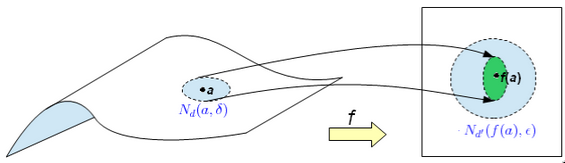
\includegraphics[width=0.8\textwidth]{assets/continuous_map_diagram.png}
  \caption{Continuous Map Diagram}
  \label{fig:continuous_map_diagram}
\end{figure}

\begin{note}
  when we say a map is continous, we mean either the map is continuous over the domain ($\forall x_0 \in X$) or that it is continuous for some specific $x_0$. For whichever case it is, it will be specified.
  \begin{enumerate}
    \item Non-continuous function: 
      \[
      D(x) = \begin{cases}
        1, x \in \Q \\
        0, \text{ else} 
      \end{cases}
      .\] 
      and $D: \R \to \R$ known as the dirichlet function
    \item Consider $f(x) = x \cdot D(x)$, this function is only only continuous at 0, $f \in C(0)$ or consider the Riemann function 
      \[
      R(x) = \begin{cases}
        \frac{1}{q}, x = \frac{p}{q} \\
        0, x \in \frac{\R}{\Q}
      \end{cases}
      .\] 
  \end{enumerate}
\end{note}

\begin{note}{Example}\\
  \begin{enumerate}
    \item  Take $f(x) = x$,  $f: [0,1] \to \R$. Without loss of generality, let $x_0 = \frac{1}{2}$ and $f(x_0) = y_0 = \frac{1}{2}$. Then, $\forall \epsilon > 0, B_{\epsilon}^{Y}(y_0) = (\frac{1}{2} - \epsilon, \frac{1}{2} + \epsilon)$ and we can take $\delta = \epsilon$ so that  $f(B_{\delta}^{X} (x_0)) = f( \left( \frac{1}{2} - \epsilon, \frac{1}{2} + \epsilon \right)) = (\frac{1}{2} - \epsilon, \frac{1}{2} + \epsilon) \subseteq B_{\epsilon}^{Y} (y_0) $.
    \item Consider 
      \begin{align*}
        f : \R &\longrightarrow \R^{2} \\
        x &\longmapsto f (x) = (x,x) 
      .\end{align*}
      this function takes the line in  $\R$ to a "diagonal" line in $\R^{2}$. 
    \item Consider 
      \begin{align*}
        g: \R^{2} &\longrightarrow \R \\
        (x,x) &\longmapsto g((x,x)) = x^{2} 
      .\end{align*}
  \end{enumerate}
\end{note}

\begin{remark}{Exercise}\\
  Consider the maps and show they are continuous
  \begin{enumerate}
    \item $\left( x,y \right) \longmapsto xy$, $f: \R^{2} \to \R$ 
    \item $\left( x,y \right) \longmapsto x+y$, $f: \R^{2} \to \R$
    \item $\left( x,y \right) \longmapsto \frac{x}{y}$, $f: \R^{2} \setminus \{y=0\} \to \R $
  \end{enumerate}
\end{remark}

\begin{theorem}
  The composition of continuous maps is continous. The map  $(g \cdot f)(x) = g(f(x))$,  $x \in X$ is called the composed map where if $f: X \to Y$ and  $g: Y \to Z$, then $g \cdot f: X \to Z$ (Kind of just  follows out from set theory)
\end{theorem}

 \begin{definition}
   If $f: X \to Y$  is a continuous map at the point $x_0$, then $f \in C(x_0)$ where $C(x_0)$ is the class of all maps from  $X \to Y$ that are continuous at $x_0$
\end{definition}

 \begin{theorem}
If $f \in C(x_0)$ and  $g \in C(f(x_0))$ then $g \cdot f \in C(x_0)$.   

\begin{proof}
  Take $\epsilon > 0$ and consider the ball  $B_{\epsilon}^{Z} (z_0)$. Since $g \in C(f(x_0)), \exists \tilde{\delta} > 0$ such that 
  \[
    g\left( B_{\tilde{\delta}}^{Y} (y_0) \right) \subseteq B_{\epsilon}^{Z} (z_0)  
  .\] Similarly, since $f \in C(x_0)$ then  $\exists \delta > 0$ such that
  \[
  f\left( B_{\delta}^{X} (x_0) ) \subseteq B_{\tilde{\delta}}^{Y} (y_0) 
  .\] 
  If then follows from (1) and (2) that 
  \[
    \left( g \cdot f \right) \left( B_{\delta}^{X} (x_0) \right) = g(f\left( B_{\delta}^{X} \left( x_0 \right) ) \right) \subseteq   g\left( B_{\tilde{\delta}}^{Y} (y_0) \right) \subseteq B_{\epsilon}^{Z} (z_0)  
  .\]
  Hence this implies $g \cdot f \in C(x_0)$
\end{proof}
 \end{theorem}

\begin{theorem}
  $f: X \to Y$ is continous on $X$ (i.e. continous at all points $x_0 \in X$) $\iff$ $\forall U_{\text{open}} \subseteq Y$, then $f^{-1}(U)$ is also open in $X$. Note  $f^{-1}$ not necessarily a function.

  \begin{proof}
    $\to$ Assume  $f: X \to Y$ is continous. Take $U_{\text{open}} \subseteq Y$ and consider $f^{-1}(U) = \{x \in X \mid f(x) \in U\} $, called the pre-image. Let us prove that $f^{-1}(U)$ is open in $X$. Take  $x_0 \in f^{-1}(U)$. Then, $f(x_0) \in U$. Since $U$ is open in $Y, \exists \epsilon > 0$ such that $B_{\epsilon}^{Y} (f(x_0)) \subseteq U$. It now follows that since $f \in C(x_0)$,  $\exists \delta > 0$ such that $f(B_{\delta}^{X} (x_0))\subseteq B_{\epsilon}^{Y} (f(x_0)) \subseteq U \Rightarrow f^{-1}(U) \supseteq B_{\delta}^{X}(x_0) \Rightarrow f^{-1}(U)$ is open since this is true for any $x_0 \in f^{-1}(U)$. \\


    $\leftarrow$ Assume that $\forall U_{\text{open}} \in Y$, we have $f^{-1}(U)$ is open in $X$. Take $x_0 \in X$ and consider the corresponding point  $y_0 = f(x_0)$. Take $\epsilon > 0$ and consider the ball $B_{\epsilon}^{Y}(y_0)$. Since a ball is an open set, we can apply our assumption,
     \[
       x_0 \in f^{-1}(B_{\epsilon}^{Y} (y_0))_{\text{open}} \subseteq X
     .\] 
Since $f^{-1}(B_{\epsilon}^{Y} (y_0))$ is open, $\exists \delta > 0$ such that 
\[
B_{\delta}^{X} (x_0) \subseteq f^{-1}(B_{\epsilon}^{Y} (y_0)) \Rightarrow f(B_{\delta}^{X} (x_0)) \subseteq B_{\epsilon}^{Y} (f(x_0))
.\]
Hence, $f \in C(x_0)$ and since this is true from any  $x_0 \in X$, $f \in C(X,Y)$.
  \end{proof}
 \end{theorem}

 \begin{theorem}
   Let $f:X \to Y$ be a continous map and $K_{\text{compact}} \subseteq X$. Then $f(K) \subseteq Y$ is compact in $Y$. 

    \begin{proof}
      Assume $f: X \to Y$ is continuous and  $K_{\text{compact}} \subseteq X$. Let $\{U_{\alpha}\}_{\alpha \in T} $ be an open cover of $f(K)$. Consider the set of open sets in  $X$ (by theorem 2):
      \[
      \{f^{-1}(U_{\alpha})\}_{\alpha \in I} 
      .\]
 Then this is an open cover of $K$,  $\cup_{\alpha \in I} f^{-1}(U_{\alpha}) \supseteq K$ (since for any $U_\alpha$ we can take  $x_0 \in f^{-1}(U_{\alpha}) \subseteq X$ and this will be true for all $x_0$). Take $x_0 \in K$,  $f(x_0) \in f(K)$ and since  $\{U_{\alpha}\}_{\alpha \in I} $ is a cover of $f(K) \exists \beta \in I$ such that 
 \[
 f(x_0) \in U_{\beta} \Rightarrow x_0 \in f^{-1}(U_{\beta})
 .\] 
 Since $K \subseteq X$ compact,  $\exists \alpha_1, \ldots, \alpha_N \in I$ such that 
 \[
 \cup_{j=1}^{N} f^{-1} (U_{\alpha_j}) \supseteq K
 .\]
 Then $\{U_{\alpha_j}\}_{j=1}^{N}$ is a finite subcover of $f(K)$,
  \[
 \cup_{j=1}^{N} U_{\alpha_j} \supseteq f(K)
 .\] Take $y_0 \in f(K)$ then  $y_0 = f(x_0), x_0 \in K$ then $\exists x_0 \in f^{-1}(U_{\alpha_{j_0}}) \Rightarrow f(x_0) \in U_{\alpha_{j_0}}$  
    \end{proof}
    \end{theorem}

 \begin{remark}
   (However, the preimage of a compact set is not necessarily compact). If $f: X \to Y$ is continuous and  $K$ is compact in $Y$ then  $f^{-1}(K)$ is not necessarily compact in $X$. Consider
    \[
      f(x) = \sin x, f: \R \to \R, K= [-1,1], f^{-1}(K) = \R \text{ not compact} 
   .\] 
 \end{remark}

 \begin{theorem}
   Let $f:X \to \R$ be a continuous map and $X$ is compact then  $\exists x_m, x_M \in X$ such that $f(x_m) = \inf_{X} f = \inf\left( \{f(x) \mid  x\in X\}  \right) $ and $f(x_M) = \sup_{X} f$. 

   \begin{proof}
     Since $X$ is compact and $f:X \to \R$ is continuous $\Rightarrow$  $im(f(X)) \subseteq \R$ is compact from the previous theorem (theorem 4), so $f(X)$ is bounded and closed. Let $\alpha = \sup_{X} f$ (this $\alpha \in \R$ exists since $\{f(x) | x \in X\} $ is bounded in $\R$). If $\alpha \in f(X)$ then  $\alpha = f(x_M)$ for some $x_M \in X$. If $\alpha \not\in f(X)$, then  $\alpha$ must be a limit point of  $f(X)$. Since  $f(X)$ is closed, $\Rightarrow d \in f(X)$, a contradiction. Hence, $\alpha \in f(X)$ and there must exist some  $f(x_m) = \inf_X f$. A similar argument can be made for the  $\sup_X f$.\\
   \end{proof}
 \end{theorem}
\end{document}
